\documentclass[12pt]{article}

\usepackage[left=2.5cm,right=2cm,top=2cm,bottom=2cm]{geometry}
\setlength{\parindent}{0mm}

\usepackage{float}
\usepackage{subfigure}

\usepackage{parskip}
\usepackage[document]{ragged2e}
\usepackage{babel}
\usepackage[utf8]{inputenc}
\usepackage{amsmath,amsthm,mathtools}
\usepackage{amsfonts,amssymb,latexsym}
\usepackage{enumerate}
\usepackage[dvips,usenames]{color}
\definecolor{RojoAnayelRey}{rgb}{1,.25,.25}
\usepackage{tikz}
\usepackage[bookmarks=true,
            bookmarksnumbered=false, % true means bookmarks in 
                                     % left window are numbered                         
            bookmarksopen=false,     % true means only level 1
                                     % are displayed.
            colorlinks=true,
            urlcolor=cyan,
            linkcolor=blue]{hyperref}
            
\usepackage[T1]{fontenc}

\title{Ejercicios sobre la distribución $T^2$ de Hotelling}

\author{David Cabezas Berrido}

\date{}

\begin{document}
\maketitle

\section{Contraste sobre $\mu$ para $\Sigma$ desconocida}

Tenemos los datos de 20 individuos, la Altura (pulgadas) y el Peso
(libras). Suponiendo que siguen una distribución $N_2(\mu,\Sigma)$ con
$\Sigma$ matriz definida no negativa, queremos contrastar las
hipótesis:

\[H_0:\quad \mu=
  \begin{pmatrix}
    70 \\ 170
  \end{pmatrix}=\mu_0;\qquad H_1:\quad \mu\neq \begin{pmatrix}
    70 \\ 170
  \end{pmatrix}=\mu_0
\]

En el caso de que la matriz $\Sigma$ sea desconocida.

Obtenemos los siguientes estadísticos muestrales básicos:

\[\bar{x}=
  \begin{pmatrix}
    71.45 \\ 164.7
  \end{pmatrix} \qquad S_n=
  \begin{pmatrix}
    14.576 & 128.88 \\ 128.88 & 1441.2653
  \end{pmatrix} \qquad r_{12}=0.889\]

Introducimos estos datos en R:
\begin{verbatim}
mu0=matrix(c(70,170), nrow=2, ncol=1) # Valor de mu para la hipótesis nula
X=matrix(c(71.45, 164.7), nrow = 2, ncol = 1) # Vector de medias muestral
# Matriz de cuasi-covarianzas muestral
Sn=matrix(c(14.576,128.88,128.88,1441.2653),nrow=2,ncol=2)
p=2
N=20
n=N-1
r12=0.889 # Coeficiente de correlación muestral
\end{verbatim}

Calculamos el valor del estadístico de contraste:

\begin{verbatim}
> # Estadístico de contraste para Sigma desconocida:
> t=20*t(x-mu0)%*%solve(Sn)%*%(x-mu0)
> t
         [,1]
[1,] 24.65119
\end{verbatim}

\[t=N(\bar{x}-\mu_0)'S_n^{-1}(\bar{x}-\mu_0)=24.65119\]

Valores de comparación teóricos bajo $H_0$ a distintos niveles de significación:

\begin{verbatim}
f01=qf(0.1, 2, 18, lower.tail = FALSE)*38/18 # alpha=0.1
f005=qf(0.05, 2, 18, lower.tail = FALSE)*38/18 # alpha=0.05
f001=qf(0.01, 2, 18, lower.tail = FALSE)*38/18 # alpha=0.01
\end{verbatim}

\begin{verbatim}
> f01
[1] 5.539444
> f005
[1] 7.504065
> f001
[1] 12.69391
\end{verbatim}

\[\frac{38}{18}F_{2,28;0.1}=5.539444 ; \qquad \frac{38}{18}F_{2,28;0.05}=7.504065 ; \qquad \frac{38}{18}F_{2,28;0.01}=12.69391\]

Para los tres niveles de significación se tiene
$24.65119=t>\frac{38}{18}F_{2,28;\alpha}$, por lo que en los tres casos
rechazaríamos la hipótesis nula.

\section{Regiones de confianza en torno a $\mu_0$ para distintos
  valores del nivel de confianza}

\subsection{Caso de $\Sigma$ conocida}

Queremos representar la elipse de ecuación
\[U=N(x-\mu_0)'\Sigma^{-1}(x-\mu_0)\]

Con $N=20$, $\mu_0=
\begin{pmatrix}
  70 \\ 170
\end{pmatrix}$ y $\Sigma=
\begin{pmatrix}
  20 & 100 \\ 100 & 1000
\end{pmatrix}
$. Y para los distintos valores de $U$:
\[\chi^2_{2;0.1}=4.60517;\quad \chi^2_{2;0.05}=5.991465;\quad \chi^2_{2;0.01}=9.21034\]
que obtenemos mediante el siguiente código de R:
\begin{verbatim}
c01=qchisq(0.1,2,lower.tail=FALSE)
c005=qchisq(0.05,2,lower.tail=FALSE)
c001=qchisq(0.01,2,lower.tail=FALSE)
\end{verbatim}

Esto lo logramos con el paquete \href{https://cran.r-project.org/web/packages/ellipse/ellipse.pdf}{\texttt{ellipse}} de R.

\begin{verbatim}
library("ellipse")

# Regiones de confianza (elipses) para los distintos niveles de significación
e1<-ellipse(x=Sigma/N, centre=as.vector(mu0), t=sqrt(c01))
plot(e1, type='l', xlim=c(67,73), ylim=c(145,195), col="red",
     xlab="Altura", ylab="Peso", main="Región de confianza para nivel 0.9")
points(x=c(as.vector(mu0)[1], as.vector(X)[1]),
       y=c(as.vector(mu0)[2], as.vector(X)[2]), pch=20)
text(x=c(as.vector(mu0)[1], as.vector(X)[1]), y=c(as.vector(mu0)[2], as.vector(X)[2]),
     pos=2, offset=0.3, labels=c('mu0', 'x'), cex=0.7, font=2)
\end{verbatim}

Primero definimos la elipse con la función \texttt{ellipse}, indicando
la matriz ($\frac{1}{N}\Sigma$), el centro ($\mu_0$) y el valor de
$U$, introducimos la raíz del valor correspondiente a cada nivel de
confianza. Con esto obtenemos 100 puntos de la elipse, que dibujamos
con \texttt{plot} en color rojo, manteniendo fijo el tamaño de los
ejes para comparar fácilmente el tamaño de las distintas elipses para
los distintos valores de $\alpha$. Después representamos y etiquetamos
el centro de la elipse ($\mu_0$) y el vector de medias muestral
($\bar{x}$). Se rechaza la hipótesis nula cuando el vector $\bar{x}$
cae fuera de la elipse.

Este código representa la elipse para el nivel de confianza $1-\alpha=0.9$.
\vspace{-4mm}
\begin{figure}[H]
  \centering
  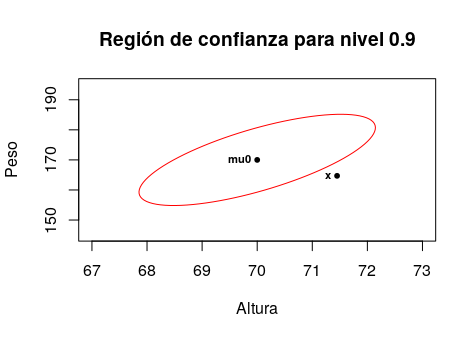
\includegraphics[width=120mm]{elipses/con-01}
  \caption{Región de confianza para el nivel $1-\alpha=0.9$. $\Sigma$ conocida.}
  \label{fig:con-01}
\end{figure}

Análogamente, los valores $\chi^2_{2;0.05}$ y $\chi^2_{2;0.01}$ nos
permiten dibujar las regiones de confianza para los niveles de
confianza $0.95$ y $0.99$ respectivamente.
\vspace{-4mm}
\begin{figure}[H]
  \centering
  \subfigure[Región de confianza al nivel $0.95$]{
    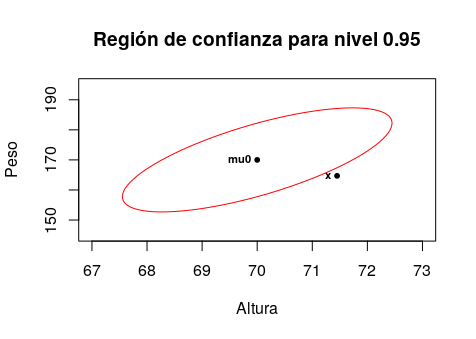
\includegraphics[width=83mm]{elipses/con-005}}
  \subfigure[Región de confianza al nivel $0.99$]{
  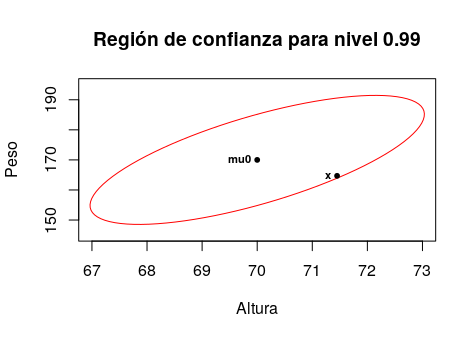
\includegraphics[width=83mm]{elipses/con-001}}
  \caption{Regiones de confianza para los niveles $0.95$ y $0.99$. $\Sigma$ conocida.}
  \label{fig:con-005-001}
\end{figure}

Nótese que la única figura en la que el vector $\bar{x}$ está dentro
de la elipse es la última (nivel de confianza $0.99$), por lo que
sería el único caso de los tres en el que no rechazaríamos $H_0$, lo
cual concuerda con los cálculos realizados en teoría.

\subsection{Caso de $\Sigma$ desconocida}

Seguimos un proceso análogo al anterior, esta vez con la ecuación
\[T^2=N(x-\mu_0)'S_n^{-1}(x-\mu_0)\]
y los valores para $T^2$:
\[\frac{38}{18}F_{2,18;0.1}=5.539444; \qquad \frac{38}{18}F_{2,18;0.05}=7.504065; \qquad \frac{38}{18}F_{2,18;0.01}=12.69391\]

Con este código en R dibujamos la primera de las elipses:
\begin{verbatim}
# Regiones de confianza (elipses) para los distintos niveles de significación
e1<-ellipse(x=Sn/N, centre=as.vector(mu0), t=sqrt(f01))
plot(e1, type='l', xlim=c(67,73), ylim=c(140,200), col="red",
     xlab="Altura", ylab="Peso", main="Región de confianza para nivel 0.9")
points(x=c(as.vector(mu0)[1], as.vector(X)[1]),
       y=c(as.vector(mu0)[2], as.vector(X)[2]), pch=20)
text(x=c(as.vector(mu0)[1], as.vector(X)[1]), y=c(as.vector(mu0)[2], as.vector(X)[2]),
     pos=2, offset=0.3, labels=c('mu0', 'x'), cex=0.7, font=2)
\end{verbatim}

\vspace{-4mm}
\begin{figure}[H]
  \centering
  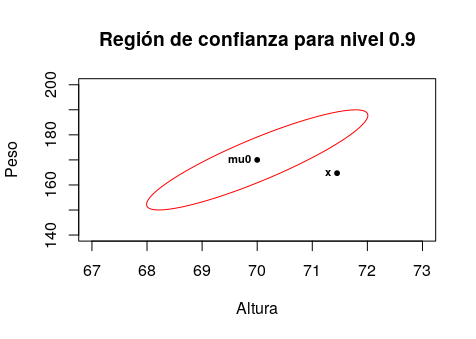
\includegraphics[width=120mm]{elipses/desc-01}
  \caption{Región de confianza para el nivel $1-\alpha=0.9$. $\Sigma$ desconocida.}
  \label{fig:desc-01}
\end{figure}

Análogamente, los valores $\frac{38}{18}F_{2,18;0.05}$ y $\frac{38}{18}F_{2,18;0.01}$ nos
permiten dibujar las regiones de confianza para los niveles de
confianza $0.95$ y $0.99$ respectivamente.
\vspace{-4mm}
\begin{figure}[H]
  \centering
  \subfigure[Región de confianza al nivel $0.95$]{
    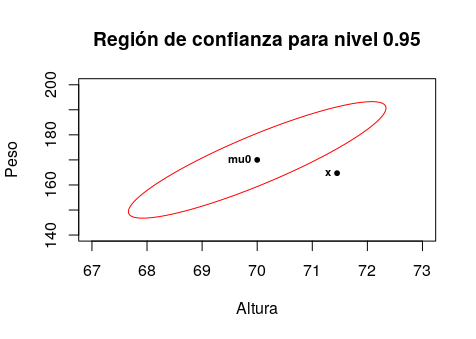
\includegraphics[width=83mm]{elipses/desc-005}}
  \subfigure[Región de confianza al nivel $0.99$]{
  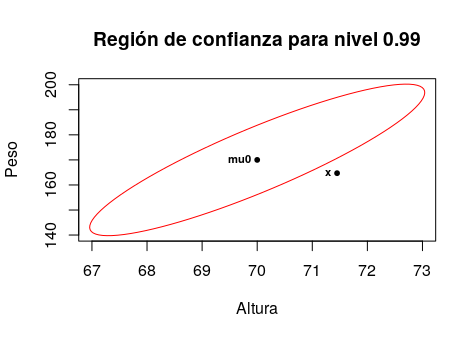
\includegraphics[width=83mm]{elipses/desc-001}}
  \caption{Regiones de confianza para los niveles $0.95$ y $0.99$. $\Sigma$ desconocida.}
  \label{fig:desc-005-001}
\end{figure}

En los tres casos, el vector $\bar{x}$ aparece fuera de la región de
confianza, por lo que rechazamos $H_0$ en todos los casos, lo que
concuerda con los cálculos realizados en el test.

\end{document}
